\documentclass{article}
\usepackage{amsfonts}
\usepackage{graphicx}
\usepackage[margin=1in]{geometry}
\usepackage{bm}
\usepackage{amsmath}
\usepackage{caption}
\usepackage{float}
\renewcommand{\familydefault}{\sfdefault}

\author{Quang P. Nguyen}
\title{Supplementary Materials}
\begin{document}
\maketitle
\captionsetup[figure]{labelfont={bf},name={Figure},labelsep=period, margin=2cm}

\section{Distribution of cILR}
\begin{figure}[h]
    \centering
    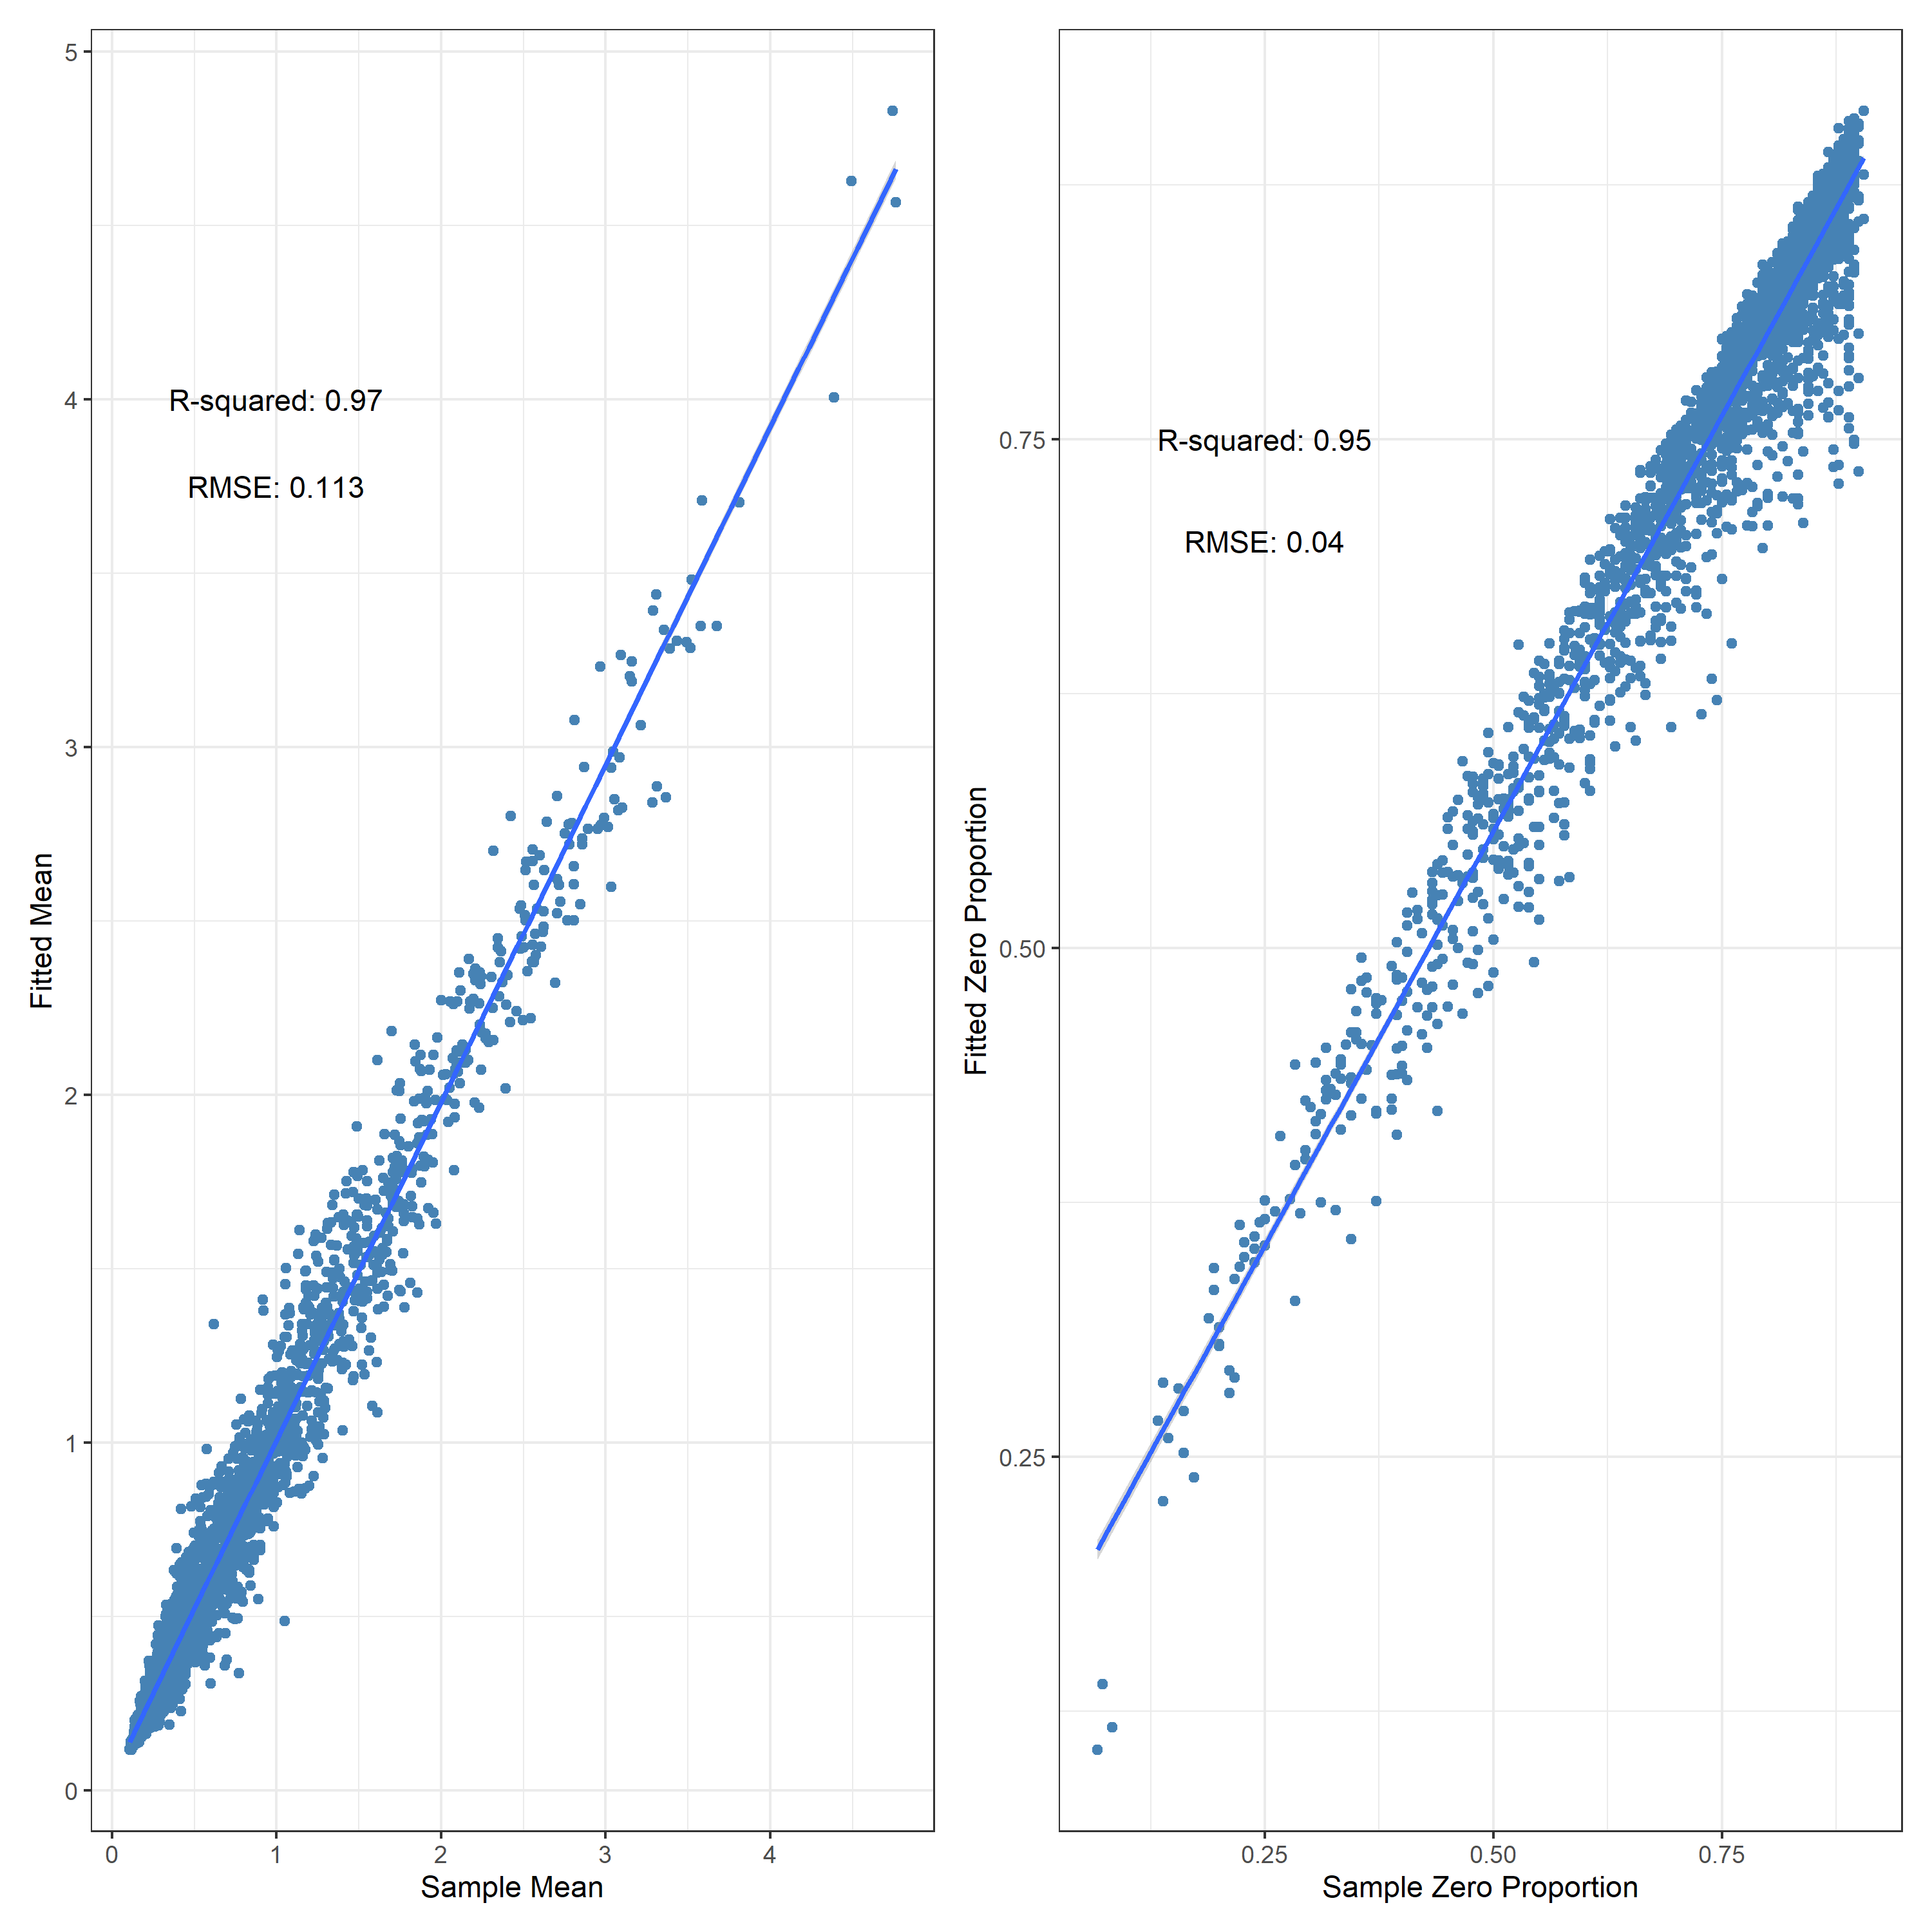
\includegraphics[width=0.8\linewidth]{figures/HMP_fit_evaluation.png}
    \caption{The distribution of cILR statistic under the null. We compared the null distribution of the test statistic and compare it with the standard normal distribution, and the t-distribution with degrees of freedom fitted to cILR scores using the maximum likelihood method}
\end{figure}

\section{Simulation Design} 

We simulated microbiome relative abundance data with flexible correlation structures using the Normal to Anything (NorTA) approach \cite{cario}. This technique can generate arbitrary multivariate continuous distributions from a target correlation structure and marginal univariate distribution. Given an $n$ by $p$ matrix of values $\mathbf{U}$ sampled from multivariate normal distribution with correlation matrix $\mathbf{\rho}$, we can generate target microbiome count vector $\mathbf{X_i}$ for taxa $i$ following distribution $\mathbf{P}$ characterized by the cumulative distribution $\mathbb{F}$:

$$X_i = \mathbb{F}^{-1}(\Phi_{U_i})$$

\noindent The negative binomial distribution was chosen as it has been shown empirically to replicate the overall distribution of non-zero microbiome count data \cite{kurtz2015}. In order to simulate data as close as possible to those collected in the field, we performed maximum likelihood fit (using \emph{fitdistrplus} in R) of the negative binomial distribution to each OTU from stool 16S rRNA sequencing data from the Human Microbiome Project (HMP), accquired through via the \emph{HMP16S} package in R \cite{schiffer2019}. Figure 2 shows the distribution of the size and mean parameters for the negative binomial distribution. 

\noindent To control for overall sparsity, we randomly sample from the count matrix with probability $1 - p_0$ where $p_0$ is the overall desired level of sparsity. Differentially abundant taxa were generated with elevated means with the effect size as the multiplier. We assumed that the overall inter-taxa correlation follows an exchangable structure with correlation $\rho_{ij}$.

\subsection{Hypothesis testing at the sample level}  
\noindent To test for hypothesis testing at the sample level, we simulate microbiome counts with marginals generated from a negative binomial distribution with mean 3.05 and size 1.67 which are the median values of fitted mean and size parameters from the HMP 16S stool data. For each experiment, the enrichment of one set will be evaluated. 

\noindent For simulations to evalute type I error control, we simulated 1 data set of 20,000 samples each with 1,000 taxa per sample with no taxa being significantly enriched for each simulation condition. Models were evaluated on a candidate set with varying sizes (50, 100, 150, 200). We also varied the overall added sparsity (0.2, 0.4, 0.6, 0.8) and the degree of inter-taxa correlation within the set (0, 0.2, 0.5).  

\noindent For simulations to evaluate power, we simulated 1 data set of 20,000 samples each with 1,000 taxa per sample for each simulation condition. Models were evaluated on a candidate set with set size of 100 taxa, enriched across all samples under different effect sizes (1.5, 2, 2.5, 3). We also varied the overall added sparsity (0.2, 0.4, 0.6, 0.8) and the degree of inter-taxa correlation within the set (0, 0.2, 0.5). 

\noindent For simulations of power and AUC classification capacity, we simulated 10 data sets of 1,000 samples each with 1,000 taxa for each simulation condition. We evaluated enrichment for one candidate set with size of 50 taxa per set.  per sample with one set of 50 taxa being significantly enriched in either all samples (power evaluation) or half the samples (AUC evaluation). We varied the overall sparsity (0.2, 0.4, 0.8), the correlation (0, 0.2, 0.5) and the effect size (1.5, 2, 2.5, 3).



\begin{figure}[h]
    \centering
    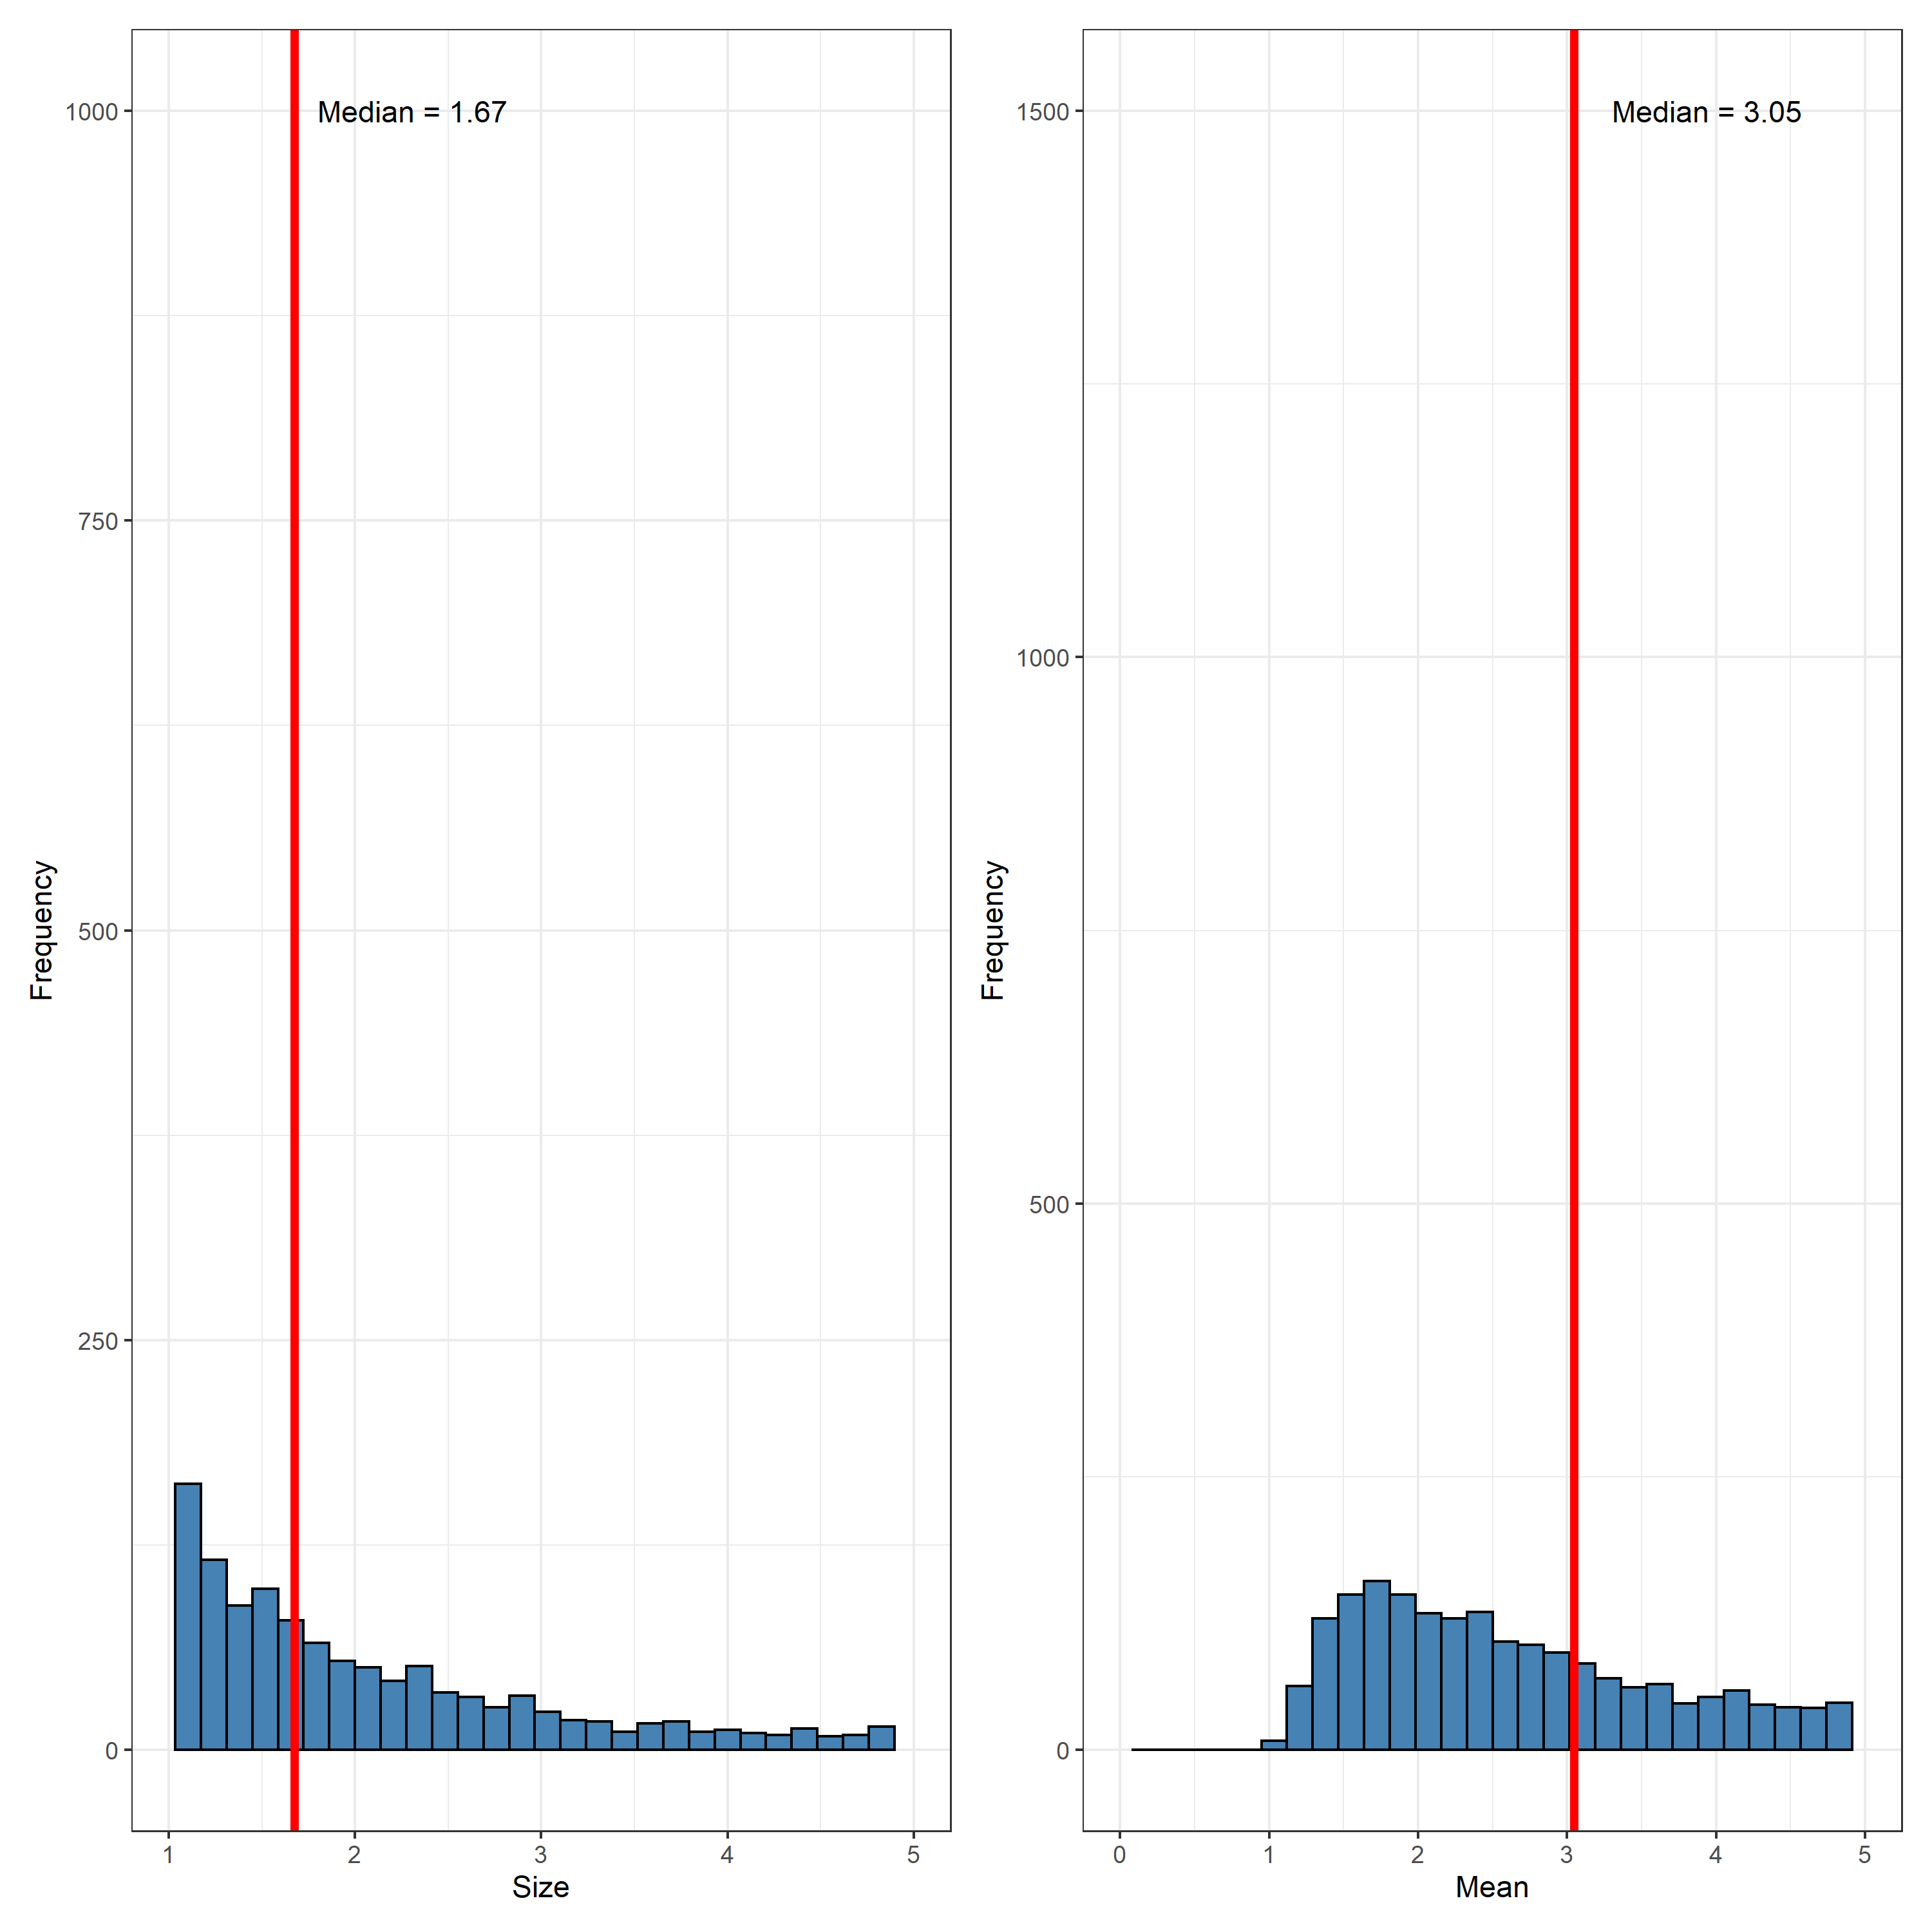
\includegraphics[width=0.6\linewidth]{figures/HMP_fit_nonzero.png}
    \caption{Distribution of each parameter of the zero inflated negative binomial distribution fitted to non-zero values of \emph{HMP16S} data. The parameters are size (panel A) and mean (panel B).}
\end{figure}


\newpage
\bibliography{tax_agg}{}
\bibliographystyle{plain}

\end{document}